\documentclass{beamer}
\mode<presentation>
\usepackage{amsmath}
\usepackage{amssymb}
%\usepackage{advdate}
\usepackage{adjustbox}
\usepackage{subcaption}
\usepackage{enumitem}
\usepackage{multicol}
\usepackage{mathtools}
\usepackage{listings}
\usepackage{url}
\def\UrlBreaks{\do\/\do-}
\usetheme{Boadilla}
\usecolortheme{lily}
\setbeamertemplate{footline}
{
  \leavevmode%
  \hbox{%
  \begin{beamercolorbox}[wd=\paperwidth,ht=2.25ex,dp=1ex,right]{author in head/foot}%
    \insertframenumber{} / \inserttotalframenumber\hspace*{2ex} 
  \end{beamercolorbox}}%
  \vskip0pt%
}
\setbeamertemplate{navigation symbols}{}

\providecommand{\nCr}[2]{\,^{#1}C_{#2}} % nCr
\providecommand{\nPr}[2]{\,^{#1}P_{#2}} % nPr
\providecommand{\mbf}{\mathbf}
\providecommand{\pr}[1]{\ensuremath{\Pr\left(#1\right)}}
\providecommand{\qfunc}[1]{\ensuremath{Q\left(#1\right)}}
\providecommand{\sbrak}[1]{\ensuremath{{}\left[#1\right]}}
\providecommand{\lsbrak}[1]{\ensuremath{{}\left[#1\right.}}
\providecommand{\rsbrak}[1]{\ensuremath{{}\left.#1\right]}}
\providecommand{\brak}[1]{\ensuremath{\left(#1\right)}}
\providecommand{\lbrak}[1]{\ensuremath{\left(#1\right.}}
\providecommand{\rbrak}[1]{\ensuremath{\left.#1\right)}}
\providecommand{\cbrak}[1]{\ensuremath{\left\{#1\right\}}}
\providecommand{\lcbrak}[1]{\ensuremath{\left\{#1\right.}}
\providecommand{\rcbrak}[1]{\ensuremath{\left.#1\right\}}}
\theoremstyle{remark}
\newtheorem{rem}{Remark}
\newcommand{\sgn}{\mathop{\mathrm{sgn}}}
\providecommand{\abs}[1]{\left\vert#1\right\vert}
\providecommand{\res}[1]{\Res\displaylimits_{#1}} 
\providecommand{\norm}[1]{\lVert#1\rVert}
\providecommand{\mtx}[1]{\mathbf{#1}}
\providecommand{\mean}[1]{E\left[ #1 \right]}
\providecommand{\fourier}{\overset{\mathcal{F}}{ \rightleftharpoons}}
%\providecommand{\hilbert}{\overset{\mathcal{H}}{ \rightleftharpoons}}
\providecommand{\system}{\overset{\mathcal{H}}{ \longleftrightarrow}}
	%\newcommand{\solution}[2]{\textbf{Solution:}{#1}}
%\newcommand{\solution}{\noindent \textbf{Solution: }}
\providecommand{\dec}[2]{\ensuremath{\overset{#1}{\underset{#2}{\gtrless}}}}
\newcommand{\myvec}[1]{\ensuremath{\begin{pmatrix}#1\end{pmatrix}}}
\let\vec\mathbf

\lstset{
%language=C,
frame=single, 
breaklines=true,
columns=fullflexible
}

\numberwithin{equation}{section}

\title{Presentation}
\author{Mohit \\ EE24BTECH11041}
\date{9 JAN 2025}
\begin{document}

\begin{frame}
\titlepage
\end{frame}

\section*{Outline}
\begin{frame}
\tableofcontents
\end{frame}
\section{Problem}
\begin{frame}
\frametitle{Problem Statement}
%
Find the roots of the following quadratic equations by factorisation.
\begin{align}
\sqrt{2}x^2 + 7x + 5\sqrt{2} = 0
\end{align}

\end{frame}

\section{Solution}
\subsection{Solution}
\begin{frame}
\frametitle{Solution}


\textbf{Theoritical Solution-}\\
Checking roots of equation exist or not,

\begin{align}
b^2 - 4ac \geq 0 \\
= 49 - 4(\sqrt{2})\brak{5\sqrt{2}}\\
= 9 
\end{align}
This means roots of equation exist.\\
And its roots are given by 
\begin{align}
x = \frac{b-\sqrt{b^2-4ac}}{2a},\frac{b+\sqrt{b^2-4ac}}{2a}\\
x = -\sqrt{2},-\frac{5}{\sqrt{2}}
\end{align}
    \end{frame}
    


\section{NEWTON-RAPHSON METHOD}
\subsection{NEWTON-RAPHSON METHOD}
\begin{frame}
\frametitle{NEWTON-RAPHSON METHOD}

Update Equation:
\begin{align}
 x_{n+1} = x_n - \frac{f(x_n)}{f'(x_n)}   
\end{align}

Steps:\\
1. Start with an initial guess $ x_0 $.\\
2. Define the function \( f(x) \) and its derivative  $f'(x)$.\\
3. Iterate using:
   \begin{align}
   x_{n+1} = x_n - \frac{f(x_n)}{f'(x_n)}
   \end{align}
   until convergence, i.e.,
   \begin{align}
   \abs{x_{n+1} - x_n} < \text{tolerance}
   \end{align}
4. Stop if $f'(x_n)$ is close to zero to avoid division by zero.
\end{frame}

\section{Plot by Finite Difference Method}
\subsection{Plot by Finite Difference Method}
\begin{frame}
\frametitle{Plot by Finite Difference Method}


\begin{figure}[h!]
   \centering
   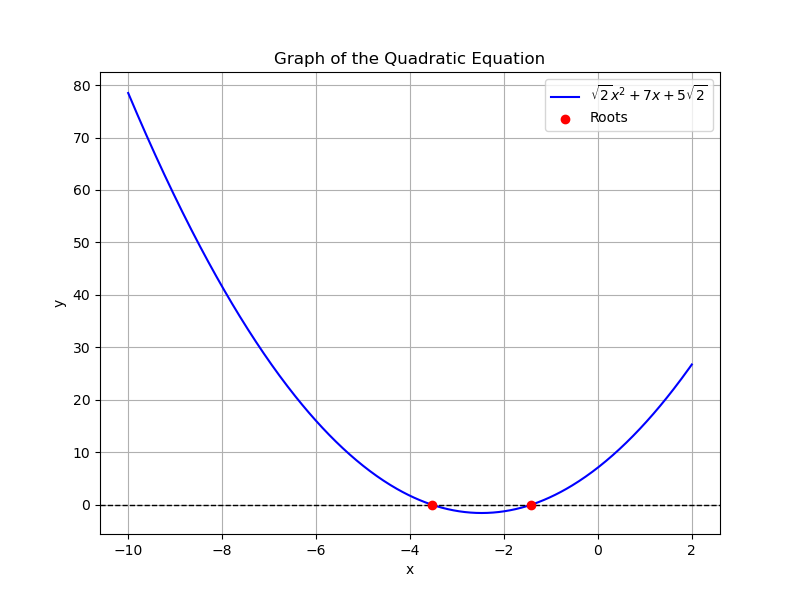
\includegraphics[width=0.7\linewidth]{figs/Figure_2.png}
   \label{Graph by Finite difference Method}
\end{figure}

\end{frame}


\section{FINDING ROOTS USING :-EIGENVALUES }
\subsection{FINDING ROOTS USING :-EIGENVALUES}
\begin{frame}
\frametitle{FINDING ROOTS USING :-EIGENVALUES}

The quadratic equation 
\begin{align}
ax^2 + bx + c = 0
\end{align}
Its Companion Matrix
\begin{align}
\text{A} =
\myvec{0 & -\frac{c}{a} \\
1 & -\frac{b}{a}
}
\end{align}
Companion matrix for $\sqrt{2}x^2 + 7x + 5\sqrt{2} = 0$
\begin{align}
\text{A} =
\myvec{0 & -5 \\
1 & -\frac{7}{\sqrt{2}}
}
\end{align}

\end{frame}


\section{QR-DECOMPOSITION:-GRAM-SCHMIDT METHOD}
\subsection{QR-DECOMPOSITION:-GRAM-SCHMIDT METHOD}
\begin{frame}
\frametitle{QR-DECOMPOSITION:-GRAM-SCHMIDT METHOD}
Let,
\begin{align}
A = QR
\end{align}
$Q$ is an $ m \times n $ orthogonal matrix\\
$R$ is an $n \times n$ upper triangular matrix.

Given a matrix $ A = [\vec{a_1}, \vec{a_2}, \dots, \vec{a_n}] $, where each $ \vec{a_i} $ is a column vector of size $ m \times 1 $.

Normalize the first column of $A$:
\begin{align}
\vec{q_1} = \frac{\vec{a_1}}{\norm{\vec{a_1}}}
\end{align}

For obtaining each column $ \vec{a_i} $, subtract the projections of the previously obtained orthonormal vectors from $ \vec{a_i} $ :
\begin{align}
\vec{a_{i+1}} = \vec{a_i} - \sum_{k=1}^{i-1} \langle \vec{a_i}, \vec{q_k} \rangle \vec{q_k}
\end{align}

\end{frame}

\section{QR-DECOMPOSITION:-GRAM-SCHMIDT METHOD}
\subsection{QR-DECOMPOSITION:-GRAM-SCHMIDT METHOD}
\begin{frame}
\frametitle{QR-DECOMPOSITION:-GRAM-SCHMIDT METHOD}

Normalize the result to obtain the next column of $ Q $:
\begin{align}
\vec{q_i} = \frac{\vec{a_i}}{\norm{\vec{a_i}}}
\end{align}

Repeat this process for all columns of $ A $.\\
\text{  }\\
We can compute the elements of $R$ by taking the dot product of the original columns of $A$ with the columns of $Q$:

\begin{align}
    A=QR\\
    Q^\top A = Q^\top QR \\
    Q^\top A = R \quad  Q^\top Q = I
\end{align}

After, this method we will get the matrix $A$ in form of $QR$.
\end{frame}

\section{QR-ALGORITHM}
\subsection{QR-ALGORITHM}
\begin{frame}
\frametitle{QR-ALGORITHM}

Let $A_0 = A $.\\
For each iteration $ k = 0, 1, 2, \dots $:-
   We got the QR decomposition of $ A_k $, such that:
    \begin{align}
    A_k = Q_k R_k
    \end{align}
    $Q_k $ is an orthogonal matrix ($ Q_k^\top Q_k = I $).\\
  $ R_k $ is an upper triangular matrix.\\
Then,form the next matrix $ A_{k+1} $ as:
    \begin{align}
    A_{k+1} = R_k Q_k
    \end{align}
\textbf{Note:-The Eigenvalues of Matrix doesn't change in QR iteration because the orthogonal matrix $Q_k$​ preserves the lengths and angles of vectors.}
  \begin{align}
    A_0 =A_1 =A_2 = \dots = A_k
    \end{align}
Repeat Step 2 until $ A_k $ converges to an upper triangular matrix $ T $. The diagonal entries of $T$ are the eigenvalues of $A$.The eigenvalues will be the roots of the Equation.

\end{frame}



\section{Plot}
\subsection{Plot}
\begin{frame}
\frametitle{Plot}

\begin{figure}[h!]
   \centering
   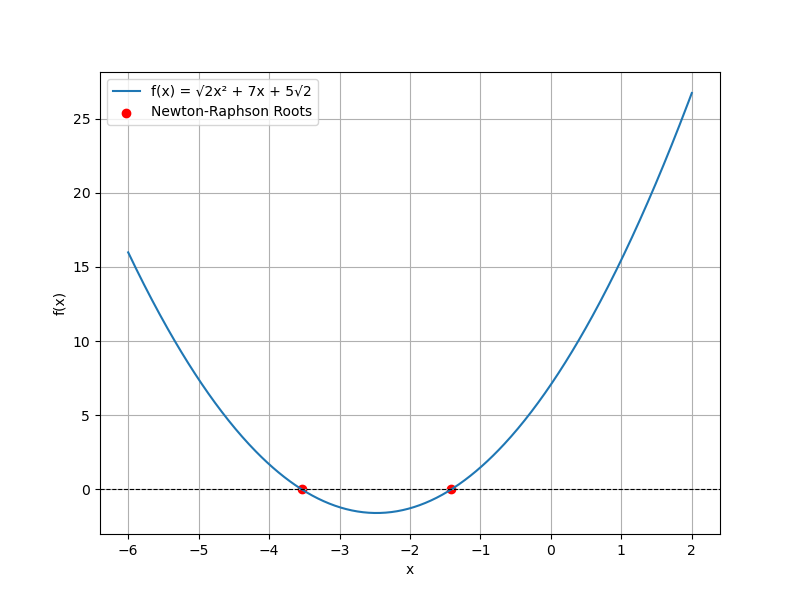
\includegraphics[width=0.7\linewidth]{figs/Figure_1.png}
\end{figure}

\end{frame}



\end{document}
